\documentclass[11pt]{article}

\usepackage[letterpaper, margin=1in]{geometry}
\usepackage{listings}
\usepackage[spanish]{babel}
\usepackage[utf8]{inputenc}
\usepackage{multirow}
\usepackage{tabularx}
\usepackage{longtable}
\usepackage{graphicx}



%Figuras
\usepackage{graphicx, subfigure}
\usepackage[]{tikz}
\usepackage{pbox}

%Matemática
\usepackage{amsmath}
\usepackage{amssymb}

%Símbolos mate extra (alfabetos, etc.)
\usepackage{mathrsfs}


%Algoritmos
\usepackage{float}
\usepackage{algorithm}
\usepackage{algorithmicx}
\usepackage{algpseudocode}
\usepackage{listings}


\usepackage{color}
\usepackage{hyperref}

\usepackage{mdframed}
\usepackage{tcolorbox}
\usepackage{multicol}
\usepackage{booktabs}
\usepackage{tabulary}
\definecolor{darkblue}{rgb}{0 , 0.054 , 0.196}



\title{Reporte de Laboratorio 4}
\author{Emmanuel Bustos - B51296 \\ Dunia Barahona - B40806}
\begin{document}

\maketitle
\hrule
\hrule
\tableofcontents
\hspace{5mm}
\hrule
\hrule


\section{Introducción}
Este laboratorio tuvo como fin enseñar al estudiante conceptos básicos de complejidad algorítmica así como el análisis de esta, su clasificación e importancia.
\subsection{Objetivos}
\begin{itemize}
	\item Aprender acerca de la complejidad algorítmica y sus tipos.
	\item Obtener la habilidad de analizar un código para obtener su función de tiempo y su complejidad algorítmica.
\end{itemize}

\section{Pregunta 1: Reseña histórica sobre los problemas NP, NP-hard y NP-complete}
\subsection{Problemas NP}
Los problemas NP, como indican Sanjeev Arora y Boaz Barak en su libro Computational Complexity: A Modern
Approach (2007), son problemas que se les puede verificar una solución de una manera efectiva en una máquina no determinista de Turing y dicha verificación posee una función de tiempo y complejidad de carácter polinomial.
\subsection{Problemas NP-hard}
Son problemas que son, al menos igual de difíciles que el más difícil de los problemas en la clase de problemas NP. Dichos problemas no son necesariamente problemas NP. Jeff Erikson (2014).
\subsection{Problemas NP-complete}
Por último, los problemas NP-complete son los problemas que son NP y NP-Hard a la vez. Se sabe que si se encuentra una solución polinomial para un problema NP-complete, existirá una solución polinomial para cada problema NP-complete. Jeff Erikson (2014).

\subsection{Diagrama de los diferentes problemas NP}

\begin{figure}[!ht]
	\caption{Diagrama de relación de los problemas NP, NP-hard y NP-complete}
	\centering
	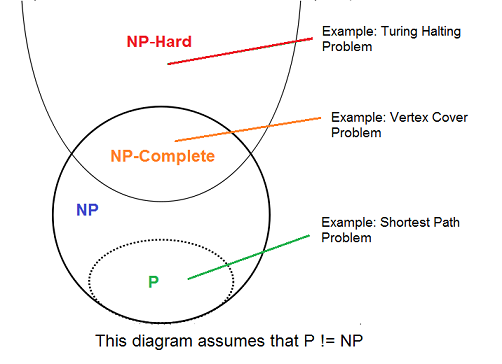
\includegraphics[width=0.5\textwidth]{1}
\end{figure}

\section{Pregunta 2: Problemas típicos}
\subsection{Problema: factorización entera}
Un problema típico de carácter NP que a su vez es NP-hard y por ende NP-complete es la factorización de un número entero en números enteros más pequeños.
\subsection{Problema: Isomorfismo entre grafos}
Es un problema de carácter NP-complete que busca determinar si dos grafos dados son isomórficos.
\subsection{Problema: Problema del viajante}
El problem es un problema de carácter NP-hard y plantea lo siguiente: Dada una lista de ciudades, y la distancia más corta entre cada una de ellas, cuál es el camino más corto para que n viajero pase por todas las ciudades y regrese a la ciudad de origen.

\section{Pregunta 3: ¿Qué hace el programa ttt.src?}
Es un programa del conocido juego "tic tac toe", también conocido como "gato", el cual crea una matriz nxn y está constantemente verificando si alguno de los dos jugadores ganó o si quedaron empate. En el programa hay una clase llamada Tictactoe, con su respectivo constructor, una función que corresponde a la función de los movimientos que vayan a realizar los jugadores, y un main.

\section{Pregunta 4: Obtener la función de tiempo y la complejidad del programa ttt.src}
\subsection{Análisis correspondiente del código}
\begin{lstlisting}
public class TicTacToe {
int[][] matrix;									
#asignacion (1)
/** Initialize your data structure here. */
public TicTacToe(int n) {						
matrix = new int[n][n];
#asignacion (1) acceso a memoria (1)
}
/** Player {player} makes a move at ({row}, {col}).
@param row The row of the board.
@param col The column of the board.
@param player The player, can be either 1 or -1.
@return The current winning condition, can be either:
0: No one wins.
1: Player 1 wins.
-1: Player 2 wins. */
int move(int row, int col, int player) {
#declaracion de la funcion nada
matrix[row][col]=player;
#acceso a memoria (1) asignacion(1)					
//check row
boolean win=true;
#asignacion y declaricion(2)
for(int i=0; i<matrix.length; i++){
#asignacion (2) comparacion(1) incremento(1), que se ejecuta n veces matrix.length veces
if(matrix[row][i]!=player){
#comparacion (2) 
#no lo tomo x no ser el peor de los casos
win=false;
#asignacion (1)
break;
#(1)
}
}
if(win) return player;
#(1) return no es el peor de los casos
//check column
win=true;
#asignacion (1)
for(int i=0; i<matrix.length; i++){
#asignacion (2) comparacion(1) incremento(1) que se ejecuta n veces
if(matrix[i][col]!=player){
#comparacion(1) acceso a memoria(1)
win=false;
#(1)
break;
#(1)
}
}
if(win) return player;
#(1) return no es el peor de los casos
//check back diagonal
win=true;
#asigancion (1)
for(int i=0; i<matrix.length; i++){
#asignacion (2) comparacion(1) incremento(1)
        if(matrix[i][i]!=player){
#comparacion (1) acceso a memoria(2)
win=false;
#asignacion(1)
break;
#(1)
}
}
if(win) return player;
#(1) return no es el peor de los casos
//check forward diagonal
win=true;
#(1)
for(int i=0; i<matrix.length; i++){
#asignacion(2) comparacion(1) incremento(1) que se ejecuta n veces
if(matrix[i][matrix.length-i-1]!=player){
#(2)
win=false;
#(1)
break;
#(1)
}
}
if(win) return player;
#(1) return (1) solo una vez
return 0;
#(1)
}
int main()
{
int player = -1;
#declaracion (1) y asignacion (1)
boolean end = false;
#(2)
int n = 3;										
#(2)
int r, c, result;								
#(3)
TicTacToe ttt = new TicTacToe(n);
#(2)
while(!end)
#n al cuadrado
{
player *= -1
#asignacion(1) operacion(1)								
r =  randomInt(0, 3);
#asignacion (1) y lo que dure randomInt ejecutandose (1)						
c =  randomInt(0, 3);                       
#asignacion(1) y lo que dure randomInt ejecutandose (1)
result = move(player, r, c);
#asignacion(1) y lo que dure move ejecutandose (24n + 16)
if(result != 0)				
#comparacion(1) se ejecuta n al cuadrado veces
#solo una vez va a entrar
{
print("player " + result + " won.");
#(1)
end = true;								
#asignacion (1)
}
}
return 0;
#(1)	
}
}
\end{lstlisting}

\subsection{Pregunta 5: Función de tiempo y complejidad}
Sumando todas las entradas correspondientes al peor de los casos en el análisis del código, se obtiene la siguiente función de tiempo: $24n^{3}+21n^{2}+17$.
Aplicándole a dicha función de tiempo la función O grande de Landeau, se obtiene que la complejidad del programa es de $n^{3}$.


\section{Conclusiones}
Con ayuda de este laboratorio, se obtuvo una clara noción de los diferentes problemas computacionales existentes, así como su comportamiento y relación mútua. Por otro lado, también se aprendió la importante habilidad de analizar un código para obtener tanto su función de tiempo como su complejidad.




\end{document}
